% Created 2018-07-11 Wed 15:29
% Intended LaTeX compiler: pdflatex
\documentclass[11pt]{article}
\usepackage[utf8]{inputenc}
\usepackage[T1]{fontenc}
\usepackage{graphicx}
\usepackage{grffile}
\usepackage{longtable}
\usepackage{wrapfig}
\usepackage{rotating}
\usepackage[normalem]{ulem}
\usepackage{amsmath}
\usepackage{textcomp}
\usepackage{amssymb}
\usepackage{capt-of}
\usepackage{hyperref}
\date{\today}
\title{}
\hypersetup{
 pdfauthor={},
 pdftitle={},
 pdfkeywords={},
 pdfsubject={},
 pdfcreator={Emacs 26.0.91 (Org mode 9.1.13)}, 
 pdflang={English}}
\begin{document}

\tableofcontents

\section{Innovationsmanagement}
\label{sec:org96c96d7}
\subsection{Technologischer Wandel \& Wettbewerbsfähigkeit}
\label{sec:org57292ba}
\begin{itemize}
\item Ausgangsproblem = Optimale Ergiebigkeit der Betriebsmittel
\item Technischer Fortschritt \& Innovationsmanagement
\begin{itemize}
\item Grundkategorien: Forschung, Entwicklung, Innovationsmanagement
\item Aufgaben der Forschung, Entwicklung \& Konstruktion
\item Aufgaben \& Ziele des Innovationsmanagements
\end{itemize}
\item Innovation \& Wettbewerbsfähigkeit
\begin{itemize}
\item Wettbewerb um F+E-Leistungen
\item Erfolgsfaktoren von Innovationen
\end{itemize}
\end{itemize}

\subsubsection{Optimale Ergiebigkeit der Betriebsmittel}
\label{sec:org47b10c9}
Betriebsmittel sind die gesamte technische Apparatur, deren sich ein Unternehmen bedient, um Sachgüter herzustellen oder Dienstleistungen bereitzustellen. Hinsichtlich der \emph{technischen Basis} kann man das Leistungspotential der Betriebsmittel abhängig vom \emph{Grad der Modernität}, \emph{Grad der Abnutzung} und dem \emph{Zustand an Betriebsfähigkeit} feststellen.

Technische Eignung 
\begin{itemize}
\item = das Verhältnis zwischen der vom Betriebsmittel verlangten \& der mit ihm tatsächlich erzielbaren Leistung
\item \emph{Wirkungsgrad}: Maximalkapazität, Minimalkapazität, Optimalkapazität, Kapazitätsreserven
\item \emph{Auslastungsgrad}: Ausschöpfung des qualitativen Leistungspotentials
\item \emph{Flexibilitätsgrad}: Universalmaschinen, Sondermaschinen, betriebstechnische Elastizität/Umstellungsaufwand
\end{itemize}

\subsubsection{Forschung, Entwicklung und Innovation}
\label{sec:orga0093c0}
\emph{Technischer Fortschritt} bezeichnet die Veränderung und zugleich technische Verbesserung von Produktionsfaktoren, Produktionsprozessen und Produkten \(\rightarrow\) Aufrechterhaltung der technologischen Wettbewerbsfähigkeit.

\emph{Forschung} und \emph{Entwicklung} beschreibt die systematische Gewinnung neuer wissenschaftlicher und technischer Erkenntnisse, mit deren Hilfe die unternehmerischen Ziele besser als bisher erreicht werden.
\begin{itemize}
\item Grundlagenforschung, angewandte Forschung
\item Forschung, Entwicklung + Konstruktion
\end{itemize}

Eine \emph{Innovation} bezeichnet eine technische Verbesserung von Produktionsfaktoren, Produktionsprozessen und Produkten, die einen Neuheitswert besitzt und für deren Angebot eine Nachfrage besteht.

\subsubsection{Aufgaben in der Forschung und Entwicklung}
\label{sec:org06be7ec}
\begin{figure}[htbp]
\centering
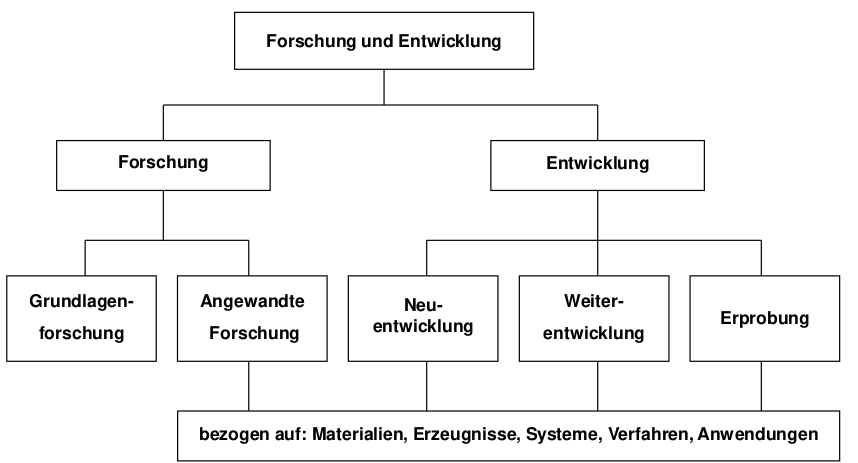
\includegraphics[width=250px]{./pictures/inaufg.png}
\caption{Aufgabenfelder}
\end{figure} 

\subsubsection{Dimensionen der Innovation}
\label{sec:org0dd95b9}
Wenn in der Betriebswirtschaftslehre von \emph{Innovationen} gesprochen wird, sind allgemein Veränderungen gemeint, die einen Neuheitswert (eine Neuartigkeit) besitzen. Mit Innovationen wird sowohl der Prozess als auch sein Ergebnis bezeichnet, wofür die Eigenschaft der Neuartigkeit zutrifft.
\begin{itemize}
\item qualitativ neuartige Produkte oder Verfahren, die sich ggü einem Vergleichszustand "merklich" unterscheiden
\begin{itemize}
\item Produktinnovationen, Produktionsverfahreninnovationen, Anwendungsinnovationen
\item Marktinnovationen (Erschließung neuer Märkte)
\item sonstige Innovatioen (Qualitätsverbesserung, sowie schnellere Bearbeitung oä)
\end{itemize}
\end{itemize}

Neuheitsgrad
\begin{itemize}
\item Ausprägung der Neuheit zu einem bestimmten Zeitpunkt
\item Invention (Erfindung), Imitation, Variation/Modifikation
\end{itemize}

Neuheitsumfang
\begin{itemize}
\item subjektiv empfundener Verlust (Nutzenschwund) der Neuheit im Zeitverlauf
\item Veränderung mit dem Lebenszyklus einer Neuheit
\item Schwund, Alterung, Verfall
\end{itemize}

Neuheitswert
\begin{itemize}
\item Messung der Vorteilhaftigkeit (Bewertung) von Innovationen im Wettbewerb
\end{itemize}

Dimensionen von Innovationen
\begin{itemize}
\item Inhaltlich: Was ist neu?
\begin{itemize}
\item Produkt, Prozess, System
\item Kontinuität, Diskontinuität
\end{itemize}
\item Intensität: Wie neu?
\begin{itemize}
\item Neu der Tatsache nach oder Neu dem Grade nach
\item Typologie von Innovationen, Multi-Dimensionalität
\end{itemize}
\item Subjektivität: Neu für wen?
\item Prozessual: Wo beginn, wo endet die Neuerung?
\begin{itemize}
\item Invention, Innovation, Imitation, Variation, Routine
\item Phasen zur Innovation
\end{itemize}
\item Normativ: Ist neu gleich erfolgreich?
\end{itemize}

\subsubsection{Aufgaben \& Ziele des Innovationsmanagements}
\label{sec:org02fa27a}
Merkmale von Innovationen
\begin{itemize}
\item systematisierte Suchprozesse nach neuen Ideen
\item schwache Strukturiertheit der  Innovationsprozesse
\item "reifende Prozesse"
\item innerbetriebliche, zwischenbetriebliche, behördliche \& protestbedingte Widerstände
\end{itemize}

Planungsaufgaben
\begin{itemize}
\item Motivation zu Innovationen
\item Zielvorgaben für Innovationen
\item Definition des Innovationsproblems
\item Suche nach innovativen Alternativen
\item Bewertung \& Auswahl der Innovationsprozesse (-projekte) und Formulierung eines Innovationsprogramms-/-budgets
\end{itemize}

Steuerungsaufaben
\begin{itemize}
\item Durchsetzung der Innovationsprozesse/Überwindung von Widerständen
\item Kontrolle der Innovationsprozesse
\item Sicherung der Innovationsprozesse und -ergebnisse
\end{itemize}

Weitere Aufgaben
\begin{itemize}
\item organisatorische Gliederung des Innovationsbereichs
\item personalpol. Aufgaben der Innovationsprojekte
\item Flexibilität der Innovationsprozesse
\end{itemize}

\subsubsection{Innovation und Wettbewerbsfähigkeit}
\label{sec:org253311b}
\begin{figure}[htbp]
\centering
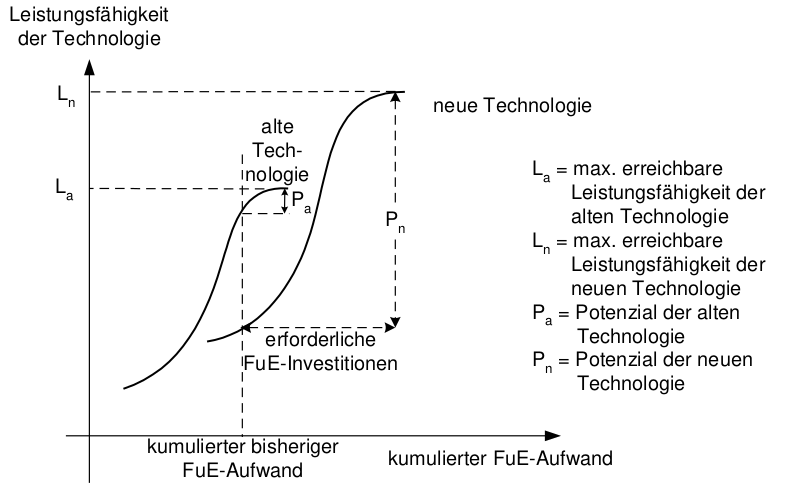
\includegraphics[width=250px]{./pictures/inskurv.png}
\caption{S-Kurven Konzept zur Technologieentwicklung}
\end{figure} 

\begin{figure}[htbp]
\centering
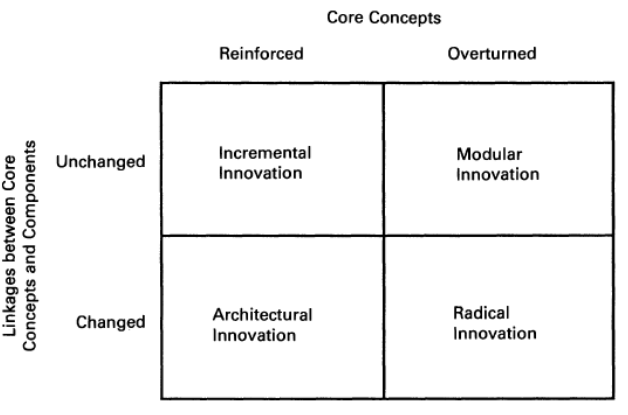
\includegraphics[width=250px]{./pictures/insfram.png}
\caption{A framework for defining innovation}
\end{figure} 

\begin{enumerate}
\item Aufgabenfelder strategischer F+E Planung
\label{sec:org85a6029}
Forschungs- und Entwicklungsprogramm
\begin{itemize}
\item Schwerpunktsetzung durch Technologiestrategie
\begin{itemize}
\item Produkt- und Prozessforschung
\item Technologien
\end{itemize}
\item Allokation des F+E-Aufwands
\end{itemize}

Eigen- oder Fremdforschung
\begin{itemize}
\item Eigenforschung zur Sicherung von Wettbewerbsvorsprüngen
\item Fremdforschung als 
\begin{itemize}
\item Auftragsforschung
\item Innovationskooperation
\item Gemeinschaftsforschung
\end{itemize}
\item Übernahme externer F+E Erkenntnisse
\begin{itemize}
\item Kauf/Lizenznahme
\item Kauf innovativer Unternehmen
\end{itemize}
\end{itemize}

\item Erfolgsfaktoren von Innovation
\label{sec:org3b8e4f2}
\begin{figure}[htbp]
\centering
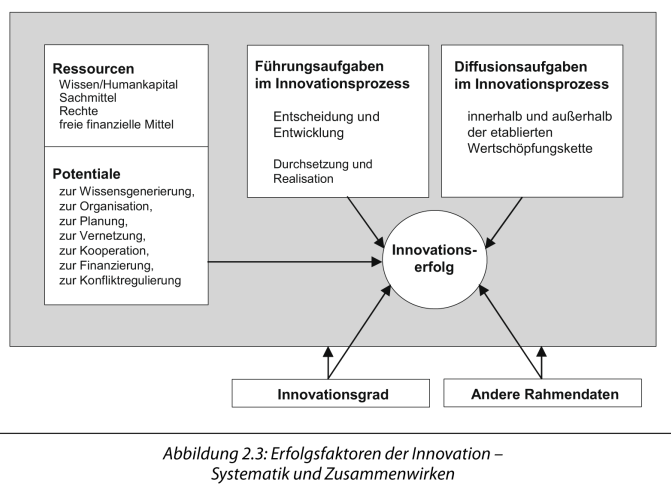
\includegraphics[width=250px]{./pictures/inerf.png}
\caption{Erfolgsfaktoren - Systematik \& Zusammenwirken}
\end{figure}
\end{enumerate}
\subsection{Strategische Forschungs- und Entwicklungsplanung}
\label{sec:org137cc06}
\subsubsection{Phasenschema des Innovationsmanagements}
\label{sec:org4ba77a2}
\begin{enumerate}
\item Planungsaufgaben der F+E
\label{sec:org3dd48e0}
Planungsaufgaben der Forschung \& Entwicklung sind:
\begin{itemize}
\item Zielbildung
\begin{itemize}
\item unter Zielbildung ist das Feststellen \& Festlegen eines präzisen, strukturierten \& realisierbaren Systems von Verhaltensnormen zu verstehen
\end{itemize}
\item Problemlücke
\begin{itemize}
\item als Problemlücke lässt sich die Abweichung der erwarteten Lage (Lageprognose) zum Soll-Zustand festlegen, die durch zielführende Maßnahmen der Entscheidungsträger geschlossen werden soll
\end{itemize}
\item Alternativensuche
\begin{itemize}
\item unter Alternativensuche ist das systematische Aufspüren, Formulieren und Analysieren von unabhängigen Vorgehensweisen zur Zielerreichung zu verstehen
\end{itemize}
\item Prognosen
\begin{itemize}
\item Prognosen sind Wahrscheinlichkeitsaussagen über das Auftreten von Ereignissen (Wirkungen, Daten) in der Zukunft, die auf Beobachtungen \& theoret. Aussagen beruhen
\end{itemize}
\item Bewertung
\begin{itemize}
\item unter Bewertung ist die Zuordnung einer Zielwirkung zu einer Alternative zu verstehen
\end{itemize}
\end{itemize}


Interdependenz von Zielbildungs- und Problemlösungsprozess
\begin{itemize}
\item \emph{Spezifität}: für Innovationen müssen spezifische Ziele formuliert werden, die Übernahme von Entscheidungen us anderen Zusammenhängen ist nicht möglich
\item \emph{Prozess}: eine Zielbildung ist kein zeitlich abgeschlossener Normsetzungsakt, sondern ein zeitverbrauchender, kognitiver \& konfliktregulierender Prozess (\emph{Reifungsprozess})
\item \emph{Parallelität}: Zielbildungsprozess \& Problemlösungsprozess verlaufen in unterschiedlichen Formen weitgehend parallel
\item \emph{Interdependenz}: Zielbildungsprozess \& Problemlösungsprozess sind wechselbezüglich verknüpft
\end{itemize}

\begin{figure}[htbp]
\centering
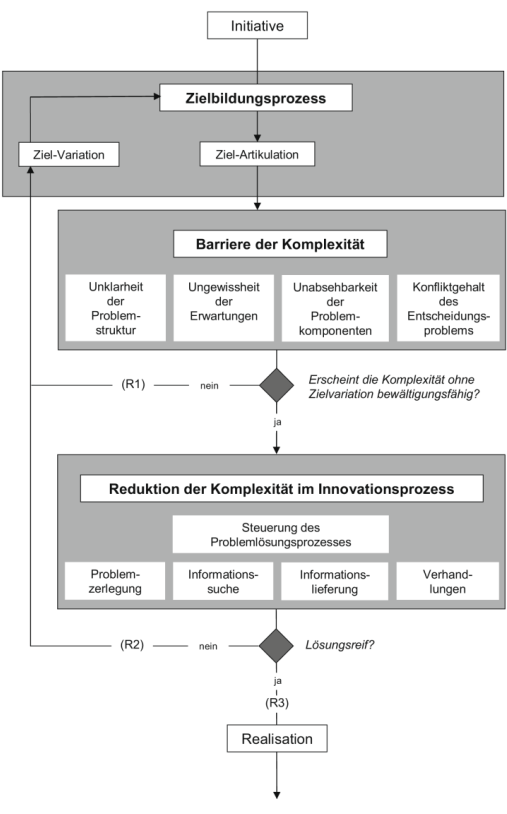
\includegraphics[width=250px]{./pictures/inziel.png}
\caption{Zielbildung im Innovationsprozess}
\end{figure} 

\item Bewertungsaufgaben der F+E
\label{sec:org923dab9}
Zielbildung
\begin{itemize}
\item unter Zielbildung ist das Feststellen \& Festlegen eines präzisen, strukturierten \& realisierbaren Systems von Verhaltensnormen zu verstehen
\end{itemize}

Bewertung
\begin{itemize}
\item Aufgaben der Bewertung:
\begin{itemize}
\item Festlegung der Bewertungskriterien \& der Kriteriengewichte
\item Ermittlung der Kriterienwerte
\item Ermittlung des Gesamtwertes der Alternative
\item Wahl der Erfolg versprechenden Forschungs- und Entwicklungsalternative
\end{itemize}
\item Aufgabe der Kontrolle
\begin{itemize}
\item Ermittlung \& Analyse von Abweichung zwischen Plangrößen (Prognose- und Vorgabegrößen) und Vergleichgrößen
\end{itemize}
\end{itemize}

\item Steuerungsaufaben der F+E
\label{sec:orgf715c87}
Steuerung
\begin{itemize}
\item als Steuerung werdne geordnete informationsverarbeitende \& zielführende Eingriffe (Anpassungsmaßnahmen) in den Realisationsprozess von Forschung \& Entwicklung definiert
\end{itemize}

Kontrolle
\begin{itemize}
\item Kontrolle ist ein geordneter, informationsverarbeitender Prozess zur Ermittlung \& Analyse von Abweichungen zwischen Plangrößen (Prognose- und Vorgabegrößen) und Vergleichsgrößen
\end{itemize}

Sicherung
\begin{itemize}
\item Sicherung umfasst alle Maßnahmen zur vorherigen Abwehr bzw. zur nachträglichen Beseitigung von Störungen bzw Fehlern im Prozess der Realisation von Forschung \& Entwicklung
\end{itemize}
\end{enumerate}
\subsubsection{Instrumente der strategischen F+E Planung}
\label{sec:org37fb8f3}
\begin{itemize}
\item Strategiche Ebene: Technologie-Portfolio
\item Taktische Ebene: Bewertungsverfahren
\item Operative Ebene: Konstruktionsbegleitende Kosten- und Leistungsrechnung
\end{itemize}

\begin{figure}[htbp]
\centering
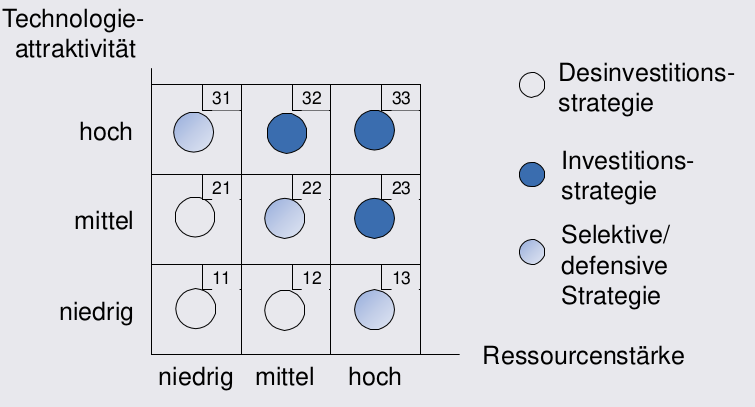
\includegraphics[width=250px]{./pictures/intechpo.png}
\caption{Technologie-Portfolio}
\end{figure} 

\begin{figure}[htbp]
\centering
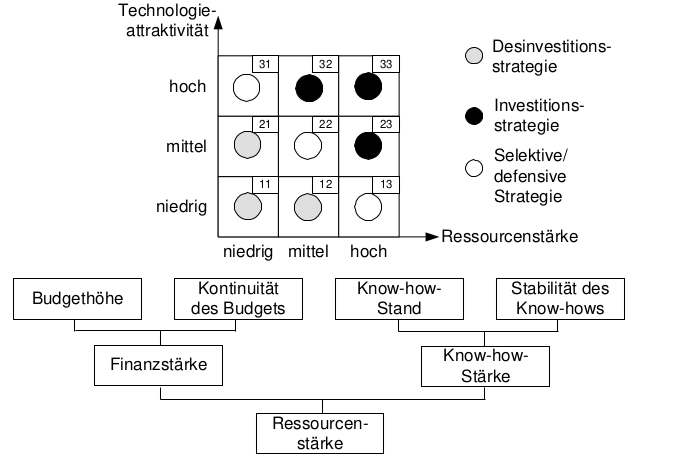
\includegraphics[width=250px]{./pictures/inrespo.png}
\caption{Ressourcenstärke \& Technologie-Portfolio}
\end{figure} 

\begin{enumerate}
\item Methoden technologischer Frühaufklärung
\label{sec:orgb7513dc}
\begin{figure}[htbp]
\centering
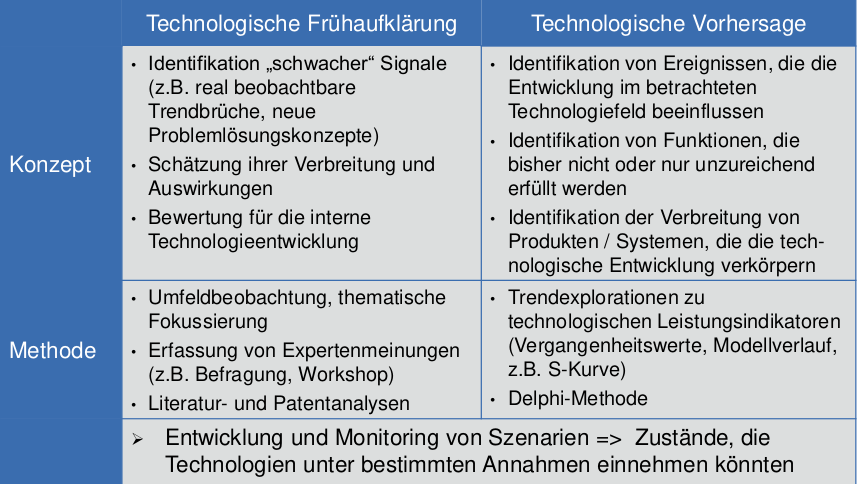
\includegraphics[width=250px]{./pictures/invor.png}
\caption{Frühaufklärung \& Vorhersage}
\end{figure}
\end{enumerate}

\subsubsection{Sicherung des Innovationswissens}
\label{sec:orgd1ad6d9}
\begin{figure}[htbp]
\centering
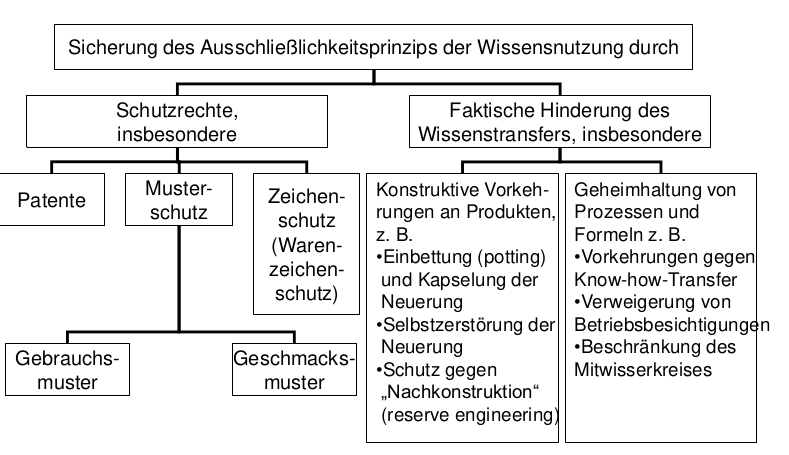
\includegraphics[width=250px]{./pictures/inauss.png}
\caption{Auschließlichkeitsprinzip zur Planung der Sicherung des Innovationswissens}
\end{figure} 

\begin{figure}[htbp]
\centering
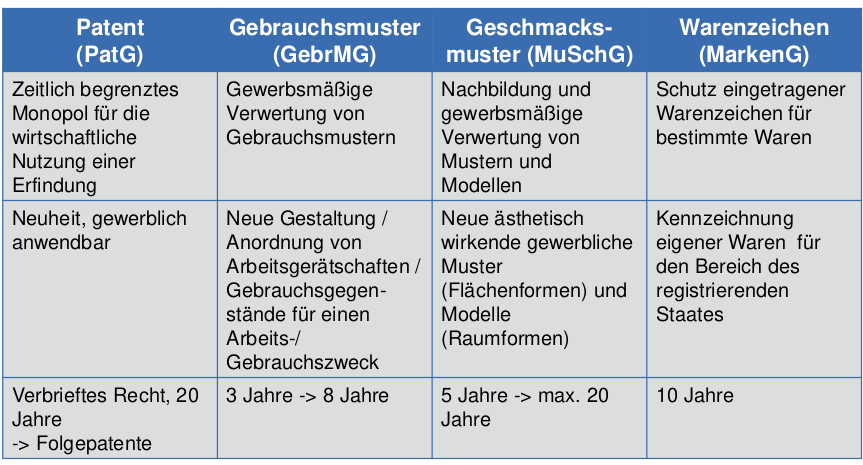
\includegraphics[width=250px]{./pictures/inmiss.png}
\caption{Rechtlicher Missbrauchsschutz}
\end{figure} 

IV\(_{\text{Innovationsmanagment}}\)\(_{\text{3.pdf}}\) F 17 Zsmfassung
\subsection{Innovationsprozesse als Managementaufgabe}
\label{sec:org9e1c5ce}
\begin{itemize}
\item nicht klausurrelevant
\end{itemize}
\end{document}
